\chapter{Элементарная работа силы и ее аналитическое выражение. Работа силы на
конечном пути. Работа равнодействующей. Мощность.}

\section{Элементарная работы силы и её аналитическое выражение}
Для характеристики действия, оказываемого силой на тело при некотором его 
перемещении, введём понятие о работе силы. Для этого введём понятие об 
элементарной работе.

\emph{Элементарной работой} силы \( \vec{F} \), приложенной к точке 
\( M \) (рис.~\ref{pic51_01}), называется скалярная величина
\[
	dA = F_\tau\,ds,
\]
где \( F_\tau \) -- проекция силы \( \vec{F} \) на касательную \( \tau \) 
к траектории точки M, направленную в сторону перемещения этой точки 
(или проекция \( \vec{F} \) на направление скорости \( \vec{v} \) точки 
\( M \)), \( ds \) -- модуль элементарного перемещения точки \( M \)).

\begin{figure}[h!]
	\center
    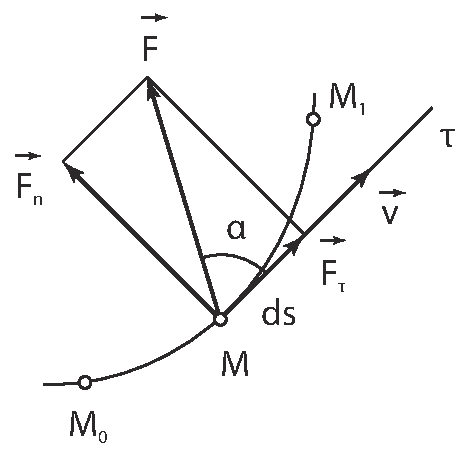
\includegraphics[width=.47\textwidth]{51_01}
    \caption{}
    \label{pic51_01}
\end{figure}

Такое определение соответствует представлению о работе как о мере того 
действия силы, которое приводит к изменению модуля скорости точки. Его можно
переписать в векторном виде:
\[
    dA = \vec{F}\cdot d\vec{r}.
\]

Следовательно, \emph{элементарная работа силы равна скалярному произведению 
силы на вектор элементарного перемещения точки и её приложения.}

Если выразить скалярное произведение через проекции векторов \( \vec{F} \) 
и \( \vec{r} \) на координатные оси и учесть, что 
\( r_x = x, r_y = y, r_z = z \), то получим \emph{аналитическое выражение 
элементарной работы}
\[
    dA = F_x\,dx + F_y\,dy + F_z\,dz,
\]
в котором \( x, y, z \) -- координаты точки приложения силы \( \vec{F} \).

\section{Работа силы на конечном пути}
Работа силы на любом конечном перемещении \( M_0 M_1 \) (рис.~\ref{pic51_01}) 
вычисляется как предел интегральной суммы соответствующих элементарных 
работ 
\[
    A_{(M_0 M_1)} = \int\limits_{(M_0)}^{(M_1)} F_\tau ds
\]
или 
\[ 
    A_{(M_0 M_1)} = \int\limits_{(M_0)}^{(M_1)} 
    \left( F_x dx + F_y dy + F_z dz \right).
\]

Следовательно, \emph{работа силы на любом перемещении \( M_0 M_1 \) равна 
интегралу от элементарной работы взятому вдоль траектории движения точки.}

Единицей измерения работы является в СИ -- джоуль.
(1 Дж = 1 Н\( \cdot \)м = 1 кг\( \cdot\text{м}^2/\text{с}^2 \)).

\section{Работа равнодействующей}
Работа, совершенная равнодействующей силой равна алгебраической сумме 
работ, совершенных отдельными силами:
\[
    A = \sum_{i=1}^{N} A_i.
\]

\section{Мощность}
Мощностью называется величина, определяющая работу, совершаемую силой 
в единицу времени. Если работа совершается равномерно, то мощность 
\( N = A/t_1 \), где \( t_1 \) -- время, в течении которого произведена 
работа \( A \). В общем случае
\[
    N = \frac{dA}{dt} = F_\tau \frac{ds}{dt} = F_\tau v = \vec{F}\cdot\vec{v}.
\]

Следовательно, \emph{мощность равна произведению касательной 
составляющей силы на скорость.}

Единицей измерения мощность в СИ является ватт (1 Вт = 1 Дж/с).

\newpage
